\section{Results}\label{sec:results}
\subsection{Equilibrium Points}\label{sec:res_equilib}
The system in study has equilibrium points when
\begin{equation}
    \begin{cases}
    -x_2-x_3 = 0&\\
    x_1 + \dfrac{100}{Ra}x_2 = 0&\\
    \dfrac{100}{R_b}\left[V_{cc0} + u(t)\right] + x_3\left(x_1 - \dfrac{100}{R_c}\right)=0&
    \end{cases}
\end{equation}
After carrying out some algebraic procedures, it can be proved that the solution is given by
\begin{equation}
    \begin{cases}
    x_1 = \dfrac{100x_3}{R_a}&\\
    x_2 = -x_3&\\
    x_3 = \dfrac{R_a}{2R_c}\left(1\pm\sqrt{1-\dfrac{4R_c^2\left[V_{cc0}+u(t)\right]}{R_aR_b}}\right)
    \end{cases}
\end{equation}
Note the double sign in $x_3$, therefore the Rössler system has two equilibrium points. These depend on both the parameters and the input $u(t)$.
 
In this work, the same parameters studied in \cite{JS_PL} will be used. Thus, $R_a=500k\Omega$, $R_b=7500k\Omega$, $R_c=17.5439$, $V_{cc0}=15V$, $RC = 1$ and input
\begin{equation}\label{eq:refInput}
    u(t) = (1000V)H(t)
\end{equation}
where $H(t)$ is the Heaviside or step function. Therefore, the equilibrium points for the Rössler system with said parameters are
\begin{equation}\label{eq:operPoints}
    \begin{split}
        P_1(x_1,x_2,x_3)=(0.5228,-2.6140,2.6140)\\
        P_2(x_1,x_2,x_3)=(5.1772,-25.8859,25.8859)
    \end{split}
\end{equation}
In this paper, the first equilibrium point $P_1$ will be considered for the linearization. In Figure \ref{fig:yOperPoint}, the system output with initial conditions in $P_1$ is shown. Note that the system's state does not change over time, validating the equilibrium point found. This simulation was conducted using fourth-order Runge-Kutta method \cite{kutta}, with fixed step size of 0.001, $t_0=0s$ and $t_{\text{end}}=100s$.

\begin{figure}[H]
    \centering
    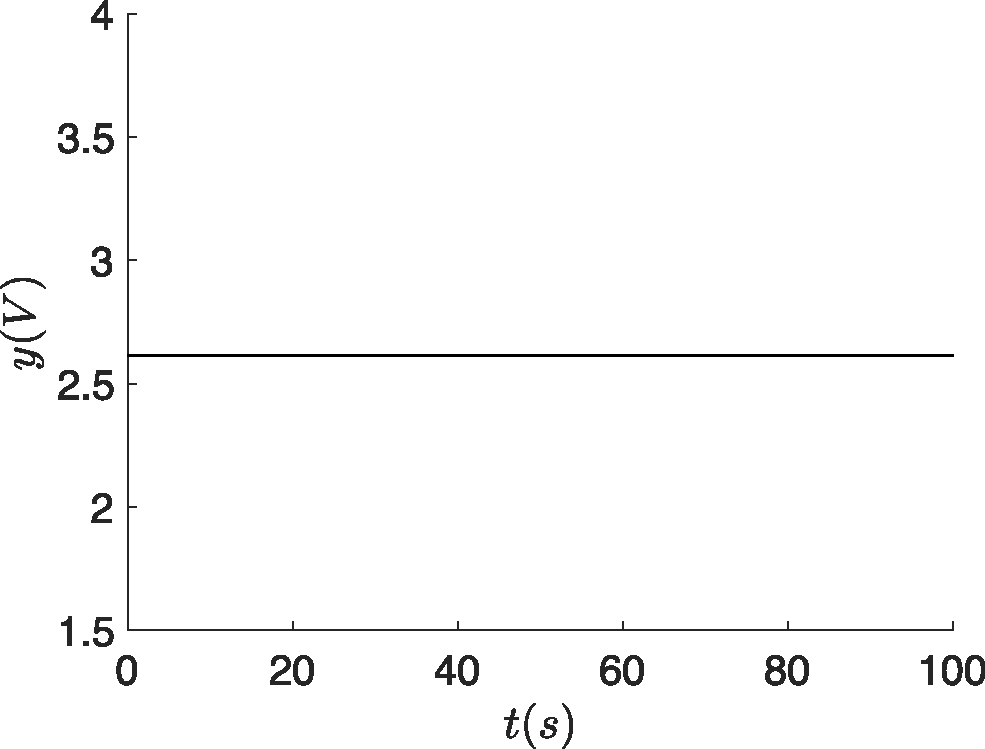
\includegraphics[scale=0.4]{figs/RosslerRquilibrium.pdf}
    \caption{System output with initial conditions at equilibrium point.}
    \label{fig:yOperPoint}
\end{figure}

\subsection{Linear Model Approximation}
For the linearization, equation (\ref{eq:state}) was used. Let $\mathbf{x}=[x_1(t)\,\, x_2(t)\,\, x_3(t)]^T$, $\mathbf{u}=u(t)$ and $\mathbf{y}=y(t)$, as the system is a SISO system. Now, the Jacobians for the linear system are
\begingroup
\renewcommand*{\arraystretch}{1.9}
\begin{equation*}
\mathbf{A} = 
\begin{bmatrix}
0 & \dfrac{-1}{RC} & \dfrac{-1}{RC}\\
\dfrac{1}{RC} &\dfrac{100}{RCR_a} & 0\\
\dfrac{x_3}{RC} & 0 & \dfrac{1}{RC}\left(x_1-\dfrac{100}{RC}\right)
\end{bmatrix}
\end{equation*}
\endgroup
\begingroup
\renewcommand*{\arraystretch}{1.3}
\begin{equation*}
\mathbf{B} = 
\begin{bmatrix}
0\\
0\\
\dfrac{100}{RCR_b}
\end{bmatrix}\quad \mathbf{C} = 
\begin{bmatrix}
0 & 0 & 1
\end{bmatrix}\quad \mathbf{D} = \begin{bmatrix}
0 
\end{bmatrix}
\end{equation*}
\endgroup
Evaluating at the operation point $P_1$ from expression (\ref{eq:operPoints}), the linear system is given by the following state space representation:
\begin{equation}\label{eq:LinearizedModel}
\begin{split}
    \Delta\mathbf{\dot{x}} =& \begin{bmatrix}
0 & -1 & -1\\
1. &0.2 & 0\\
2.614 & 0 & -5.1772
\end{bmatrix} \Delta\mathbf{x}+\begin{bmatrix}
0\\
0\\
0.0133 
\end{bmatrix}\Delta\mathbf{u}\\\vspace{5mm}
    \Delta\mathbf{y}=&\begin{bmatrix}
0 & 0 & 1
\end{bmatrix}\Delta\mathbf{x}
\end{split}
\end{equation}
The linearization was performed as well using the command \texttt{linmod} from Matlab through a simulation diagram, like \ref{fig:simulink}, in Simulink and the same results were obtained.

\subsection{Linearity Curve}\label{sec:linearityCurve}
In this section we present the linearity curve in order to compare the linear approximation with the nonlinear dynamic system in study. In Fig. \ref{fig:linearityCurve} this curve can be observed.

\begin{figure}[H]
    \centering
    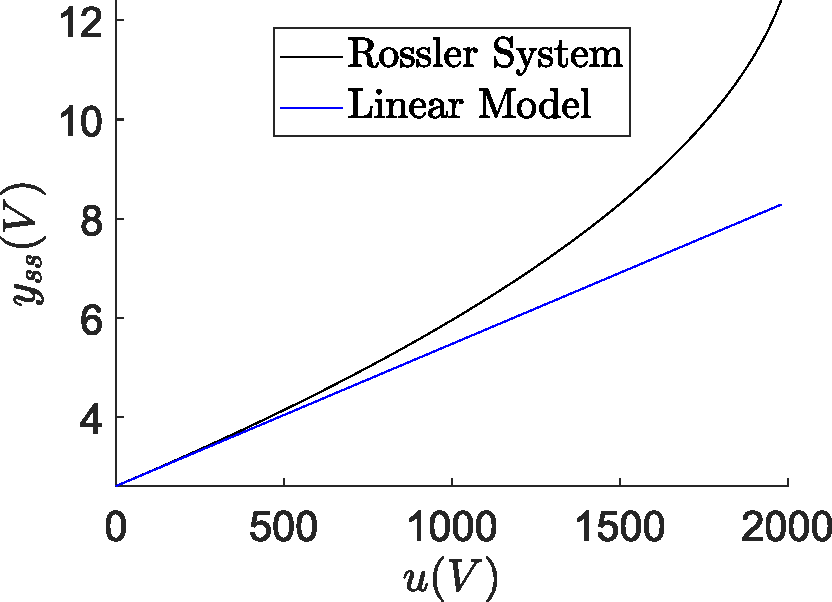
\includegraphics[scale=0.5]{figs/curvaLinealidad.pdf}
    \caption{Linearity Curve}
    \label{fig:linearityCurve}
\end{figure}

%%%%%%%%%%%%%%%%%%%%%%%%%%%%%%%%%%%%%%%%%%%%%%%%%%%

\subsection{Comparison: Linear and Nonlinear System Response}\label{sec:compar_LinearNonlinear}
In the following results, the same parameters described in section \ref{sec:res_equilib} will be used (for both the system and for the simulation).
\subsubsection{Comparison regarding the Input}
The previously selected input (equation \ref{eq:refInput}) will be changed by a factor $\varepsilon$. For the nonlinear system, the input will be 
\begin{equation*}
    u(t)=(1000V + \varepsilon)H(t)
\end{equation*}
whereas, for the linear system, the input will be
\begin{equation*}
    \Delta \mathbf{u}=\mathbf{u}-\mathbf{u_0}=(1000V + \varepsilon)H(t) - (1000V)H(t) = \varepsilon H(t)
\end{equation*}

The comparison will be performed, first, exactly at the operation point, then close to it and finally far from the initial input.

For a comparison exactly at the operation point, $\varepsilon=0V$. The results are presented in Fig. \ref{fig:comparDelta0}.

\begin{figure}[H]
    \centering
    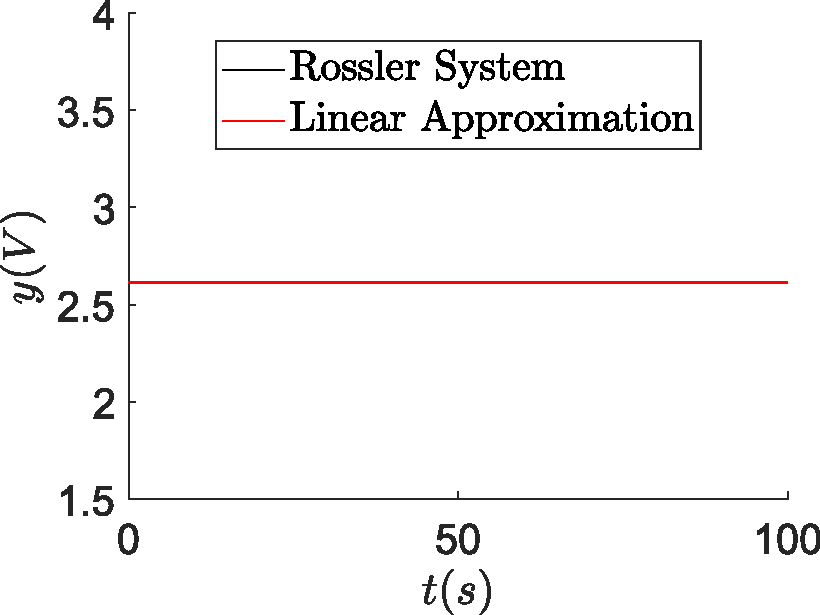
\includegraphics[scale=0.5]{figs/comparLinearVSNonlinear/yvsT_InputDelta0.pdf}
    \caption{Output for $\varepsilon=0V$.}
    \label{fig:comparDelta0}
\end{figure}

For a comparison close to the operation point, $\varepsilon=50V$. The system output is shown in Fig. \ref{fig:comparDelta50}. Note that the behaviour is almost identical.

\begin{figure}[H]
    \centering
    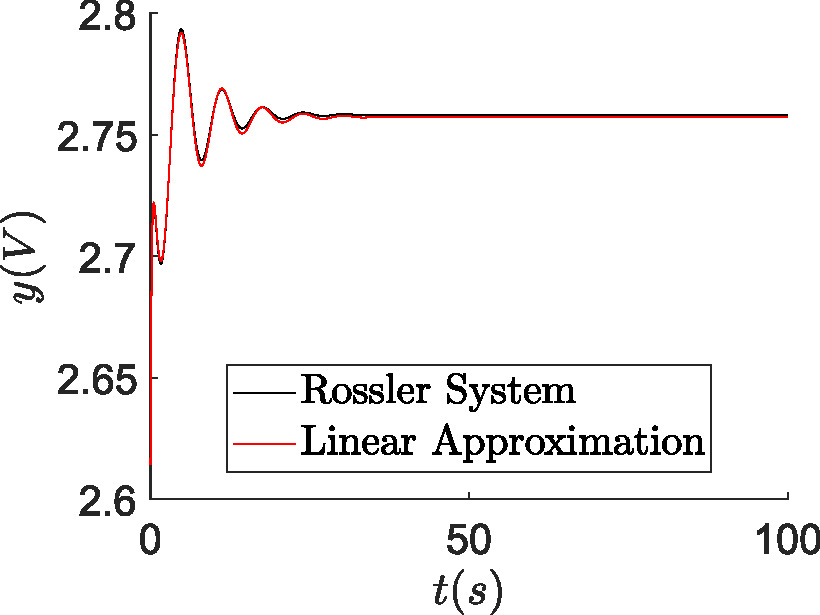
\includegraphics[scale=0.5]{figs/comparLinearVSNonlinear/yvsT_InputDelta50.pdf}
    \caption{Output for $\varepsilon=50V$.}
    \label{fig:comparDelta50}
\end{figure}

For a comparison far from the operation point, $\varepsilon=200V$. The system output is shown in Fig. \ref{fig:comparDelta200}. Note that the two systems start to differ.
\begin{figure}[ht]
    \centering
    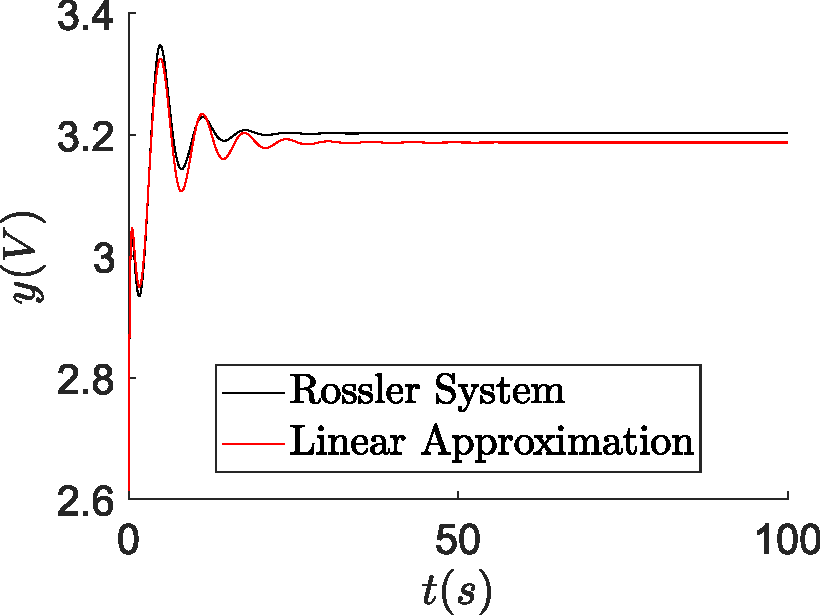
\includegraphics[scale=0.5]{figs/comparLinearVSNonlinear/yvsT_InputDelta200.pdf}
    \caption{Output for $\varepsilon=200V$.}
    \label{fig:comparDelta200}
\end{figure}

In order to show how the systems differ over time with inputs significantly far from the operation point, one last simulation will be shown. For the following results (Fig. \ref{fig:comparDelta750}), $\varepsilon=750V$ is used; note that the output is notably different: not stabilizing in the same value nor showing the same oscillation.
\begin{figure}[H]
    \centering
    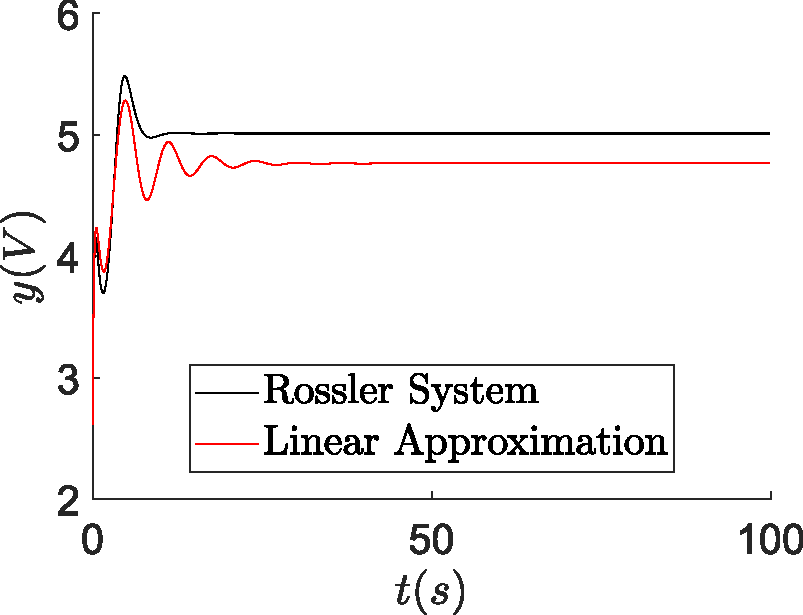
\includegraphics[scale=0.5]{figs/comparLinearVSNonlinear/yvsT_InputDelta750.pdf}
    \caption{Output for $\varepsilon=750V$.}
    \label{fig:comparDelta750}
\end{figure}

One last comparison was performed for a sine input
\begin{equation}
    u(t)=(1V)\sin(t) + 1000V
\end{equation} which yields the following input for the linear approximation:
\begin{equation}
    \Delta\mathbf{u}=(1V)\sin(t)
\end{equation}

In the following plot (Fig. \ref{fig:sinInput_compar}), the systems responses are displayed. Note that both systems overlap; it was expected that the linear model will have the same behavior only in stationary state, but, surprisingly, also in transitory state the response is reproduced.
\begin{figure}[ht]
    \centering
    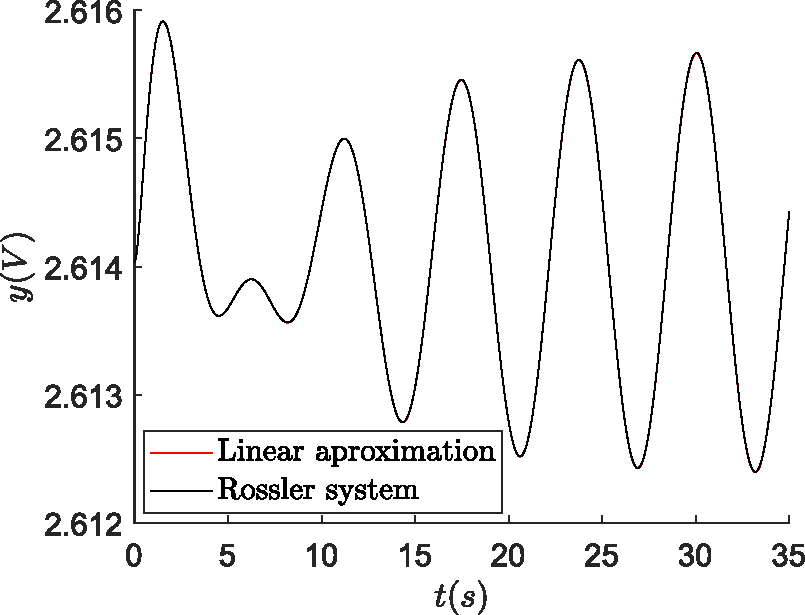
\includegraphics[scale=0.5]{figs/comparLinearVSNonlinear/Entrada_seno_lineal_no_lineal.pdf}
    \caption{Comparison between the linear and nonlinear model for a sine input.}
    \label{fig:sinInput_compar}
\end{figure}


\subsubsection{Comparison regarding the Initial Conditions} \label{sec:initCondCompar}
In this section, the initial conditions for $x_3$ will be changed using a small, medium and large factor $\varepsilon$, that is $x_3(0)=2.6140V+\varepsilon$. All simulations were performed with all same parameters from previous section, except for $t_{\text{end}}=35s$ since the system stabilizes quickly and for $t_{\text{end}}=100s$ it would show a lot of not relevant behavior.

For initial conditions close (small change) to the operation point, $\varepsilon=0.1V$. In Fig. \ref{fig:ci_x3_01} the comparison between the linear and the nonlinear is shown. Note that the change is so subtle that the output responses overlap.

\begin{figure}[H]
    \centering
    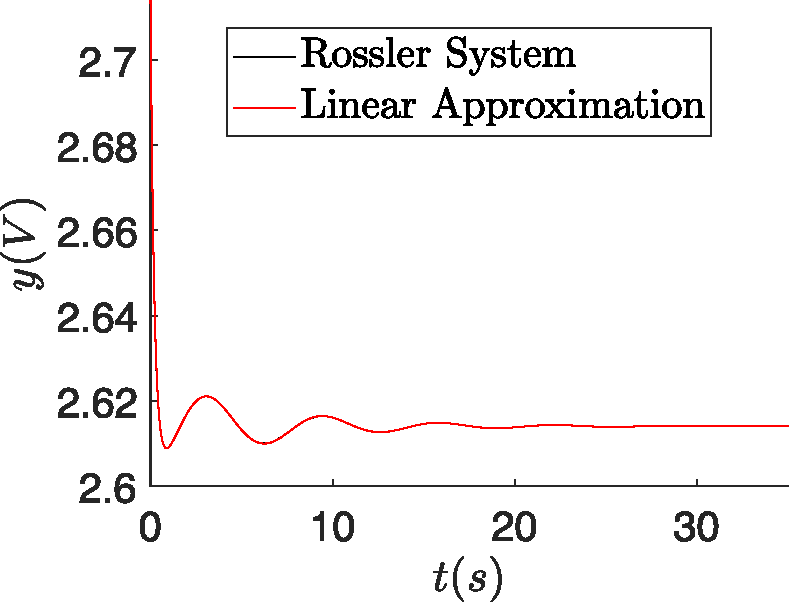
\includegraphics[scale=0.5]{figs/comparLinearVSNonlinear/Cerca_lineal_nl_01.pdf}
    \caption{Output for $\varepsilon=0.1V$ in initial conditions.}
    \label{fig:ci_x3_01}
\end{figure}


For a medium change, $\varepsilon=50V$ is considered. As it can be observed in Fig. \ref{fig:ci_x3_50}, both outputs are similar, only differing in the magnitude of each oscillation.

\begin{figure}[H]
    \centering
    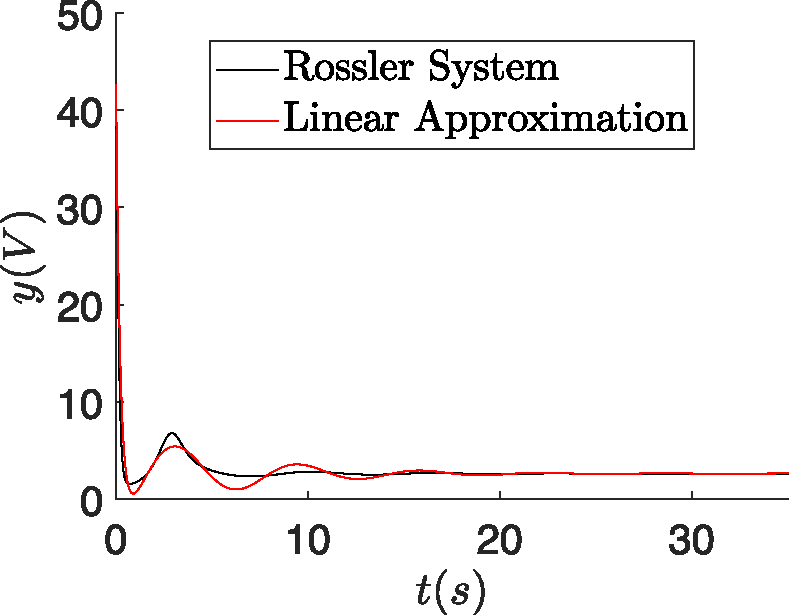
\includegraphics[scale=0.5]{figs/comparLinearVSNonlinear/Medio_lineal_nl_50.pdf}
    \caption{Output for $\varepsilon=50V$ in initial conditions.}
    \label{fig:ci_x3_50}
\end{figure}

Finally, $\varepsilon=400V$ was set for a large change in the initial conditions for $x_3$. The results are displayed in Fig. \ref{fig:ci_x3_400}. This plot shows that, at this point, both systems diverge one from another over time.
\begin{figure}[H]
    \centering
    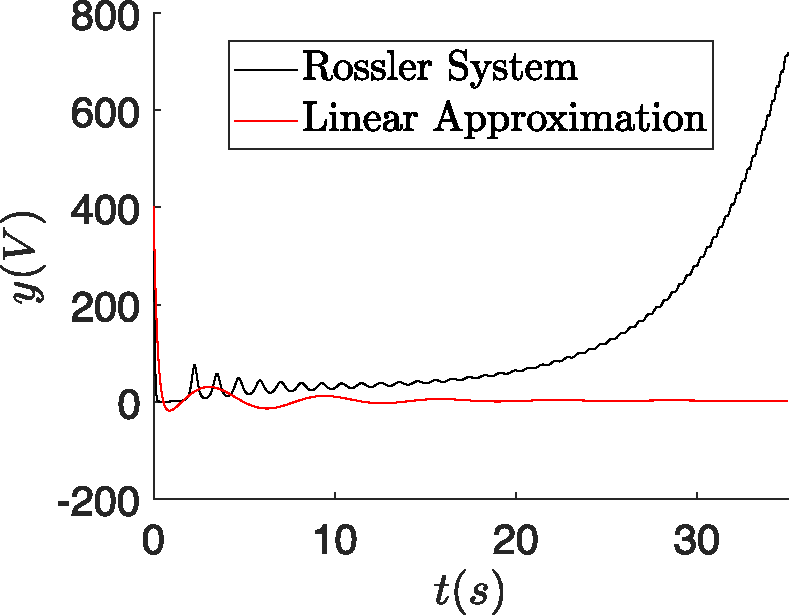
\includegraphics[scale=0.5]{figs/comparLinearVSNonlinear/Lejos_lineal_nl_400.pdf}
    \caption{Output for $\varepsilon=400V$ in initial conditions.}
    \label{fig:ci_x3_400}
\end{figure}

Two last simulations were performed changing all initial conditions and the input. For the first one, making a small change in all parameters: the input was increased by $3V$ and \textbf{each} of the initial conditions were changed by adding $0.1V$; the results for this simulation are presented in Fig. \ref{fig:Delta_all_small}. 
\begin{figure}
    \centering
    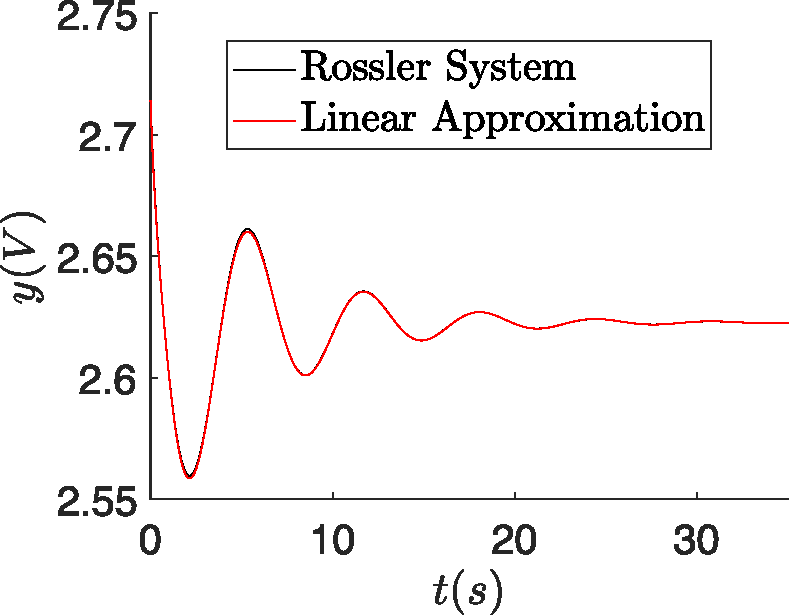
\includegraphics[scale=0.55]{figs/comparLinearVSNonlinear/Cerca_todos_lineal_nl_u3_ci01.pdf}
    \caption{Output for small changes in all parameters.}
    \label{fig:Delta_all_small}
\end{figure}

Finally, for a relatively large change in all parameters: the input was increased by $30V$ and $10V$ was added to all initial conditions. The outcome of this simulation can be seen in Fig. \ref{fig:Delta_all_large}. Note that the nonlinear Rössler system starts to show a strange behavior, which cannot be reproduced by the linear system.
\begin{figure}[ht]
    \centering
    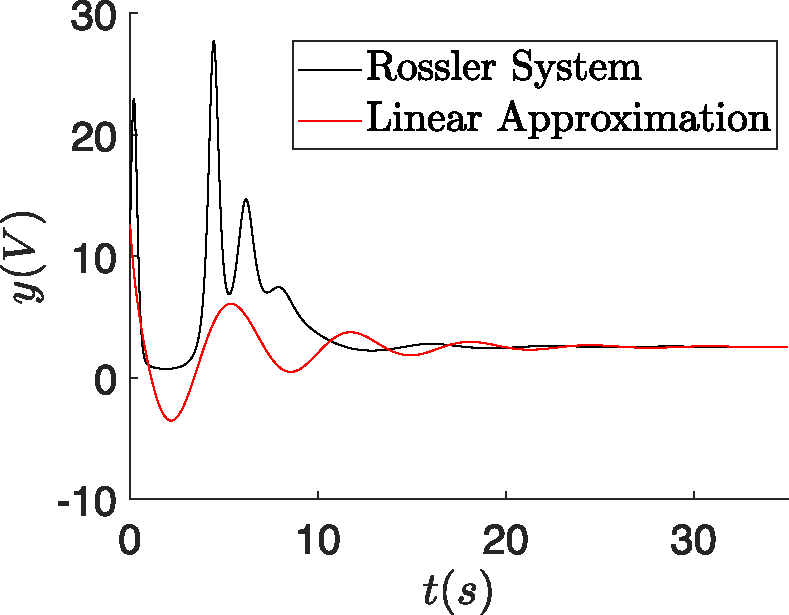
\includegraphics[scale=0.5]{figs/comparLinearVSNonlinear/Lejos_todos_lineal_nl_u30_ci10.pdf}
    \caption{Output for relatively large changes in all parameters.}
    \label{fig:Delta_all_large}
\end{figure}

%%%%%%%%%%%%%%%%%%%%%%%%%%%%%%%%%%%%%%%%%%%%%%%%%%%
\subsection{Continuous Transfer Function}\label{sec:result_tf}
 Based on the method presented in section \ref{sec:tf}, the transfer function was obtained from the linear state-space model from equation (\ref{eq:LinearizedModel}) and using equation (\ref{eq:ss2tf}), the transfer function for the linearized system is
 \begin{equation}\label{eq:tfNuestra}
     G(s)=\dfrac{0.01333s^2-0.002667s+0.01333}{s^3+4.977s^2+2.597s+4.654}
 \end{equation}
 which is the exact same equation that was calculated using \textit{Matlab}.
 
 %%%%%%%%%%%%%%%%%%%%%%%%%%%%%%%%%%%%%%%%%%%%%%%%%%%
 \subsection{Sampling Time Selection}
  The selection of sampling time for the discretization was done accordingly with was discussed in section \ref{sec:sampling}. The growth time was extracted from a simulation with the same parameters for the linealization (section \ref{sec:res_equilib}), except for the input of $u(t)=1002V$. The obtained time response is shown in Fig. \ref{fig:growth_Time} as well as the two points needed to calculate the growth time.
  
  \begin{figure}[ht]%NOOO
      \centering
      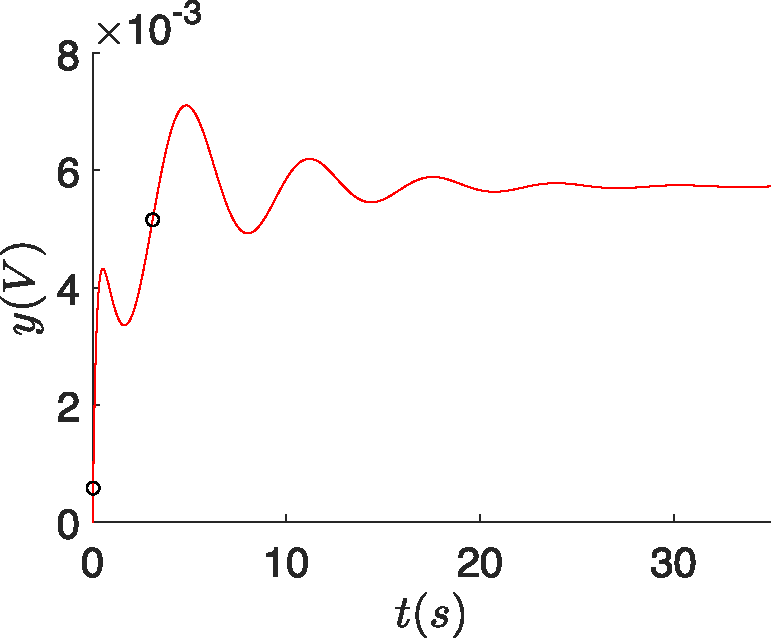
\includegraphics[scale=0.4]{figs/Growth_time.pdf}
      \caption{Time response and points for the growth time.}
      \label{fig:growth_Time}
  \end{figure}
  
  From here, it was the growth time was gotten: $T_r=3.073s$. Now applying the criterion mentioned in section \ref{sec:sampling}, the sampling time must satisfy
  \begin{equation}
      0.3073s<T<1.5365s
  \end{equation}
  Therefore, the selected sampling time for the discretization is $T=1s$.
 
 %%%%%%%%%%%%%%%%%%%%%%%%%%%%%%%%%%%%%%%%%%%%%%%%%%%
 
 \subsection{Discrete Transfer Function}
 The discretization was performed with the strategy presented in section \ref{sec:c2d} and the transfer function (equation (\ref{eq:tfNuestra})) obtained in section \ref{sec:result_tf}. The discrete transfer function is
 \begin{equation}\label{eq:tfNuestraD}
    G(z)=\dfrac{0.001906z^2-0.001946z+0.00226}{z^3-0.9395z^2+0.721z-0.006893}
 \end{equation}
 
 %%%%%%%%%%%%%%%%%%%%%%%%%%%%%%%%%%%%%%%%%%%%%%%%%%%
 \subsection{Comparison regarding the Transfer Functions and Linear Model}
 In this section, the time response of the system will be compared using three tools: the continuous (equation (\ref{eq:tfNuestra})) and discrete (equation (\ref{eq:tfNuestraD})) transfer functions and the linearized model (equation (\ref{eq:LinearizedModel})). 
 
 The simulation was performed with two inputs: a unitary step and a unitary impulse. The parameters are the same as in section \ref{sec:res_equilib}. In Figs. \ref{fig:tfsStep}-\ref{fig:tfsImpulse}
\begin{figure}[ht]
    \centering
    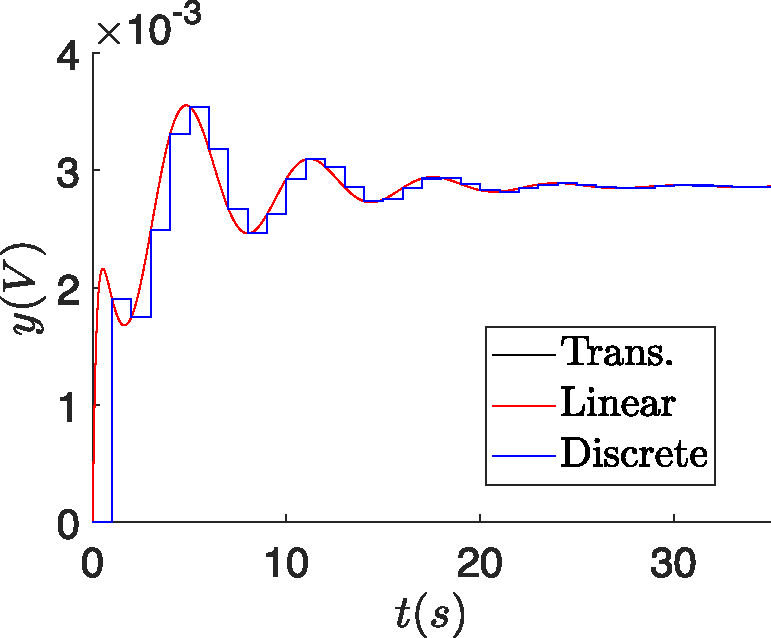
\includegraphics[scale=0.5]{figs/transferFunc/Comp_trans_lineal_unitstep.pdf}
    \caption{System's output to step input through three different methods.}
    \label{fig:tfsStep}
\end{figure}

\begin{figure}[ht]
    \centering
    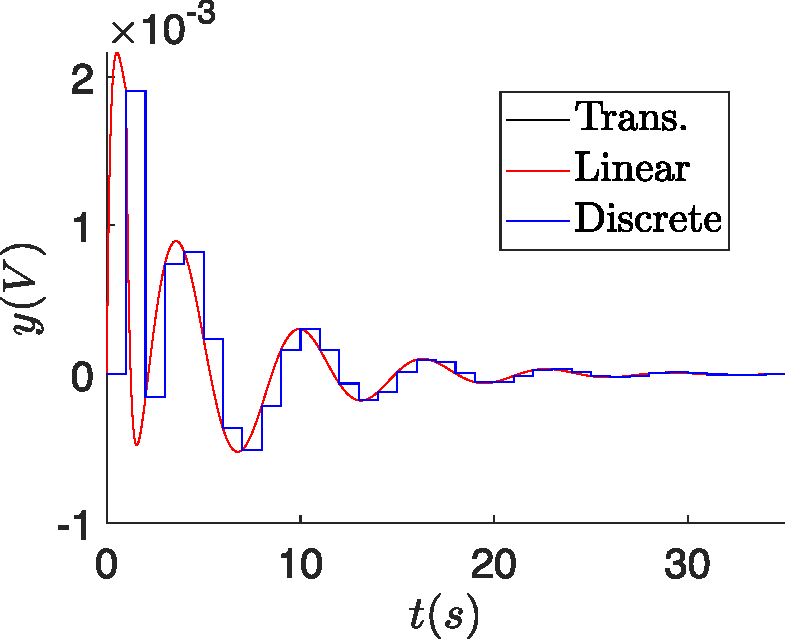
\includegraphics[scale=0.5]{figs/transferFunc/Comp_trans_lineal_impulse.pdf}
    \caption{System's output to impulse input through three different methods.}
    \label{fig:tfsImpulse}
\end{figure}
Note that in both simulations, the output through the linearized system and its respective continuous transfer function is the same, since both graphs overlap, validating the function obtained. The discrete system gives an acceptable approximation, missing out the some of the first peaks of the system.

%%%%%%%%%%%%%%%%%%%%%%%%%%%%%%%%%%%%%%%%%%%%%%%%%%%

\subsection{Ponderation Sequence}
Following the ideas of section \ref{sec:ponderationSequence}, the ponderation sequence was obtained by taking the inverse $\mathcal{Z}$-transform of the discrete transfer function (\ref{eq:tfNuestraD}), which is equivalent to calculate the system response to an unitary impulse; table \ref{tab:ponderation} shows the first 10 terms of this sequence.

\begin{table}[H]
\centering
\begin{tabular}{cc}
\hline
\boldmath$k$ & \boldmath$g(k)$ \\ \hline
0 & 0 \\
1 & 0.0019 \\
2 & -0.0002 \\
3 & 0.0007 \\
4 & 0.0008 \\
5 & 0.0002 \\
6 & -0.0004 \\
7 & -0.0005 \\
8 & -0.0002 \\
9 & 0.0002 \\ \hline
\end{tabular}
\caption{Ponderation Sequence}
\label{tab:ponderation}
\end{table}

From this values, given an input, the respective output can be calculated (as described in section \ref{sec:ponderationSequence}) using discrete convolution. The following results show the response of the discrete system through this sequence for two inputs:
\begin{align}
    u_1(k)&=H(k)\\
    u_2(k)&=\delta(k)
\end{align}
where $H$ is the Heaviside or step function and $\delta$ is a unitary impulse or Kronecker delta. The response to the first input is displayed in Fig. \ref{fig:ponderStep}, and for the second one in Fig. \ref{fig:ponderImpulse}. Notice that in both cases, for both inputs, the outputs overlap with the simulation of the original linear state-space model; note as well that the discrete output is only calculated for the 10 values of the ponderation sequence. In order to obtain more points on the curve, more points for the ponderation sequence must be calculated.
\begin{figure}[ht]
    \centering
    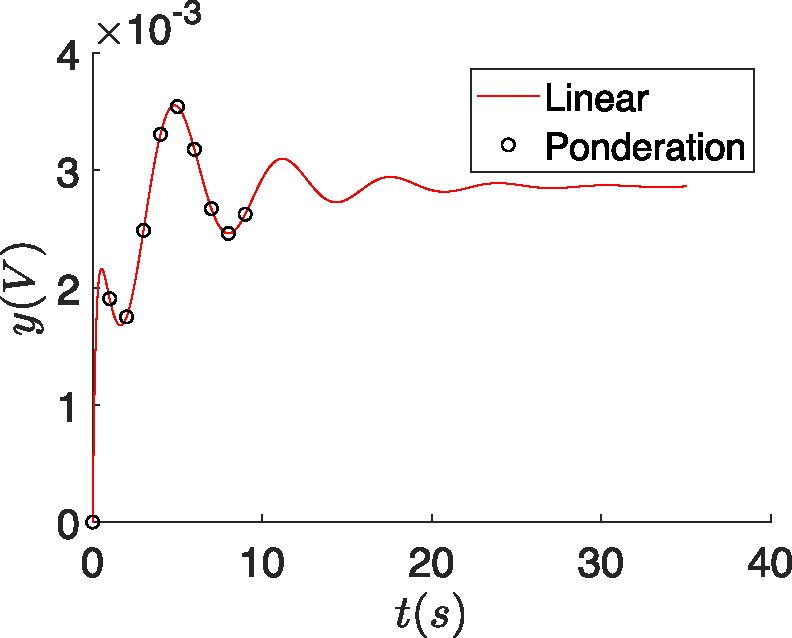
\includegraphics[scale=0.5]{figs/pondrtion/Comp_ponderation_linear.pdf}
    \caption{System output for $u_1$ using the ponderation values.}
    \label{fig:ponderStep}
\end{figure}
\begin{figure}[ht]
    \centering
    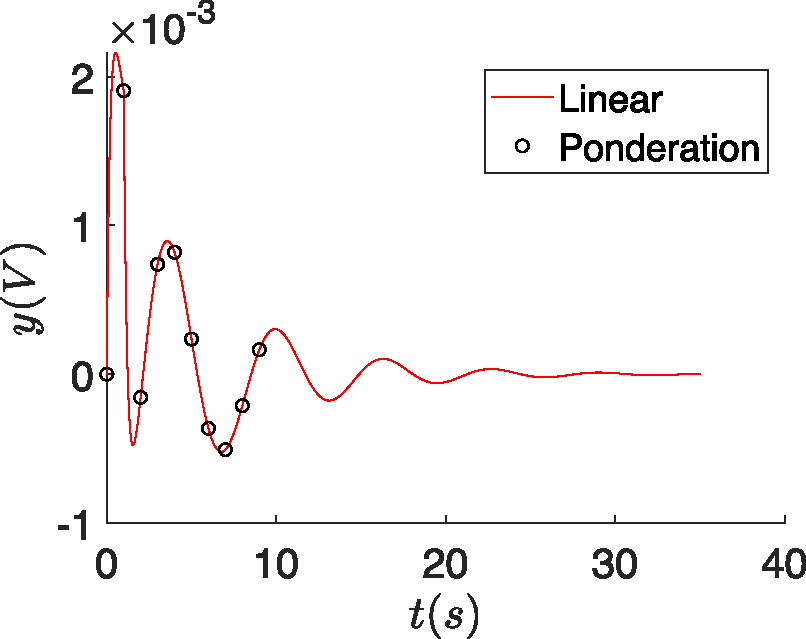
\includegraphics[scale=0.5]{figs/pondrtion/Comp_ponderation_linear_impulse.pdf}
    \caption{System output for $u_2$ using the ponderation sequence.}
    \label{fig:ponderImpulse}
\end{figure}

%%%%%%%%%%%%%%%%%%%%%%%%%%%%%%%%%%%%%%%%%%%%%%%%%%%

\subsection{Order Reduction}\label{sec:order_reduction}
This section presents the results obtained using the three methods discussed in section \ref{sec:reduct}. The poles and zeros of the transfer function (\ref{eq:tfNuestra}) will be calculated first.

The zeros of the continuous transfer function are given by the solutions to
\begin{equation}
    0.01333s^2-0.002667s+0.01333=0
\end{equation}
Therefore, $s_{z_1,z_2}=0.100\pm0.995i$ are the two \textbf{finite} zeros of the transfer function; and for the poles, the following equation must be solved:
\begin{equation}
    s^3+4.977s^2+2.579s+4.654=0
\end{equation}
which solutions are $s_{p_1,p_2}=-0.1698\pm0.9873i$ and $s_{p_3}=-4.6376$. Clearly, the first method cannot be applied; note that the two finite zeros are complex and cannot be compared directly with the poles. On the other hand, for the poles, for the same reason as the zeros, they cannot be canceled out directly, since they provide essential properties to the system such as the oscillation. Finally the pole at $s_{p_3}=-4.6376$ does not have a close zero to be canceled out with.

For the second method, the complex poles and zeros cannot be canceled out; but for the pole $s_{p_3}$, the method can be applied: the dominant pole can be considered as $\Re(-0.1698\pm0.9873i)=-0.1698$ and the pole $s_{p_3}=-4.6376$ is more than 10 times away from the dominant pole. Therefore, the reduced transfer function using the second method is 
\begin{equation}\label{eq:reduced_insignificant}
    \tilde{G}(s)= \dfrac{0.002875 s^2 - 0.000575 s + 0.002875}{s^2 + 0.3396 s + 1.004}
\end{equation}
The following plot (Fig. \ref{fig:reduced_insignificant}) shows the linear system's response to an input
\begin{equation}\label{eq:input_reduced}
    u(t)=(2V)H(t)
\end{equation}
compared with the response to the linear non-reduced system (equation (\ref{eq:tfNuestra})). In the figure it can be observed that both systems almost overlap starting from $t=2s$.
\begin{figure}[H]
    \centering
    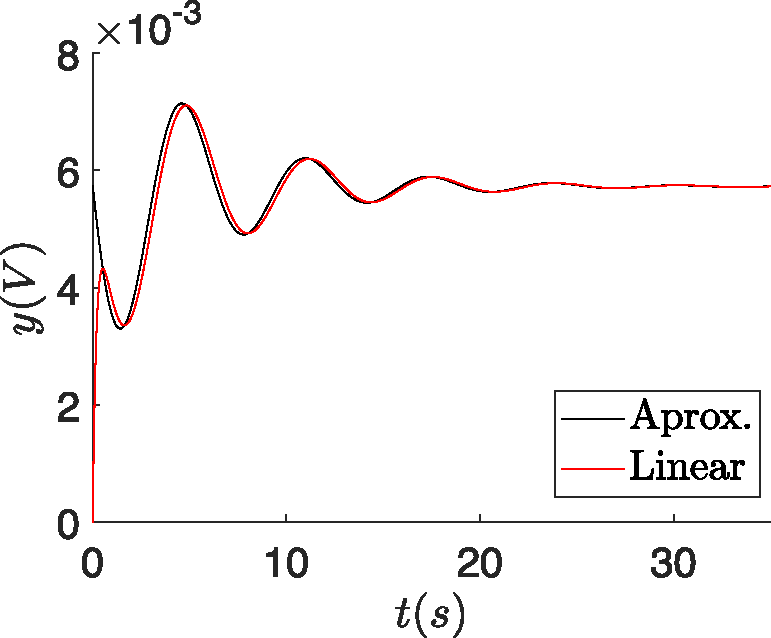
\includegraphics[scale=0.5]{figs/reduc/Reduccion_nosotros.pdf}
    \caption{Results obtained with the reduced model (\ref{eq:reduced_insignificant}).}
    \label{fig:reduced_insignificant}
\end{figure}

Next, the 2nd order approximation, presented in section \ref{sec:reduct}, was performed based on the response to the original linearization of the Rössler system, based on a response to a step input. The parameters for the transfer function were calculated: $\zeta= 0.4125$, $\omega_0=0.7144$ and $k=0.0029$. With this results, the following 2nd order transfer function was acquired:

\begin{equation}\label{eq:reduced_order2}
    \tilde{G}(s)=\dfrac{0.001461}{s^2 + 0.5887 s + 0.5102}
\end{equation}
The response of the system for an input as (\ref{eq:input_reduced}) is presented in Fig. \ref{fig:reduced_order2}. As expected, since it is an experimental approach, the results are not really good; the model successfully approximates the growth time, the maximum overshoot and the stationary state, but the oscillation frequency of the approximated system is slower than the actual model. 
\begin{figure}[H]
    \centering
    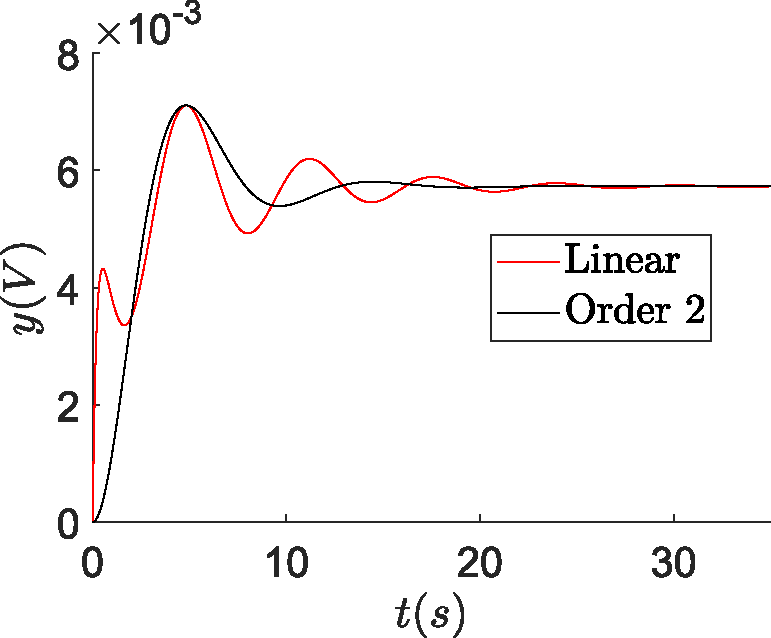
\includegraphics[scale=0.5]{figs/reduc/Red_Aprox_nosotros_orden2.pdf}
    \caption{Results obtained with the reduced model (\ref{eq:reduced_order2}).}
    \label{fig:reduced_order2}
\end{figure}

Finally, the order reduction was performed using \textit{Matlab}, with the command mentioned in section \ref{sec:reduct}. The resulting transfer function is
\begin{equation}\label{eq:reduced_matlab}
    \tilde{G}(s)=\dfrac{0.0027 s^2 - 0.0005665 s + 0.002697}{s^2 + 0.3575 s + 0.9416}
\end{equation}
The same simulation was conducted for this new transfer function, as the previous reductions, and the result can be observed in Fig. \ref{fig:reduced_matlab}.
\begin{figure}[H]
    \centering
    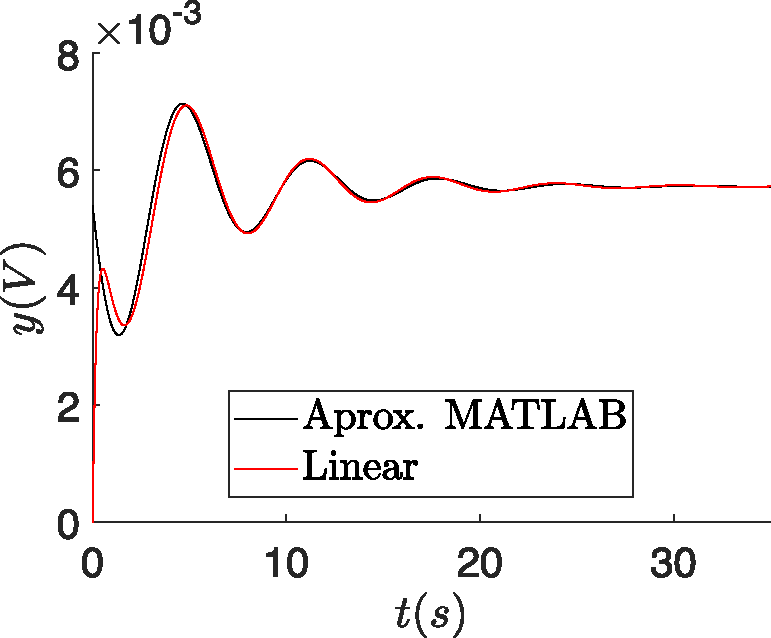
\includegraphics[scale=0.5]{figs/reduc/Reduccion_matlab.pdf}
    \caption{Results obtained with the reduced model (\ref{eq:reduced_matlab}).}
    \label{fig:reduced_matlab}
\end{figure}
This plot shows that the approximated model is just as good as the one obtained through the insignificant pole cancellation, since both graphs overlap from around $t=4s$.

%%%%%%%%%%%%%%%%%%%%%%%%%%%%%%%%%%%%%%%%%%%%%%%%%%%

\subsection{Routh-Hurwitz}
For the following stability analysis tools, the parameter $R_a$ was chosen to be analyzed. It is desired to find the region where the linear system is stable. In order to achieve this goal, the characteristic polynomial needs to be obtained in terms of the parameter $R_a$. Applying the formula $P(s)=|s\mathbf{I}-\mathbf{A}|=0$, the resulting polynomial is
\begin{equation}\label{eq:charPoly}
    \begin{split}
        R_as^3 + (5.1772R_a - 100.0)s^2 &+ (3.614R_a - 517.72)s\\
        &+ 5.1772R_a - 261.4=0
    \end{split}
\end{equation}
And the respective Routh-Hurwitz array for this polynomial is
{\renewcommand{\arraystretch}{1.6}
\begin{table}[H]
\centering
\refstepcounter{table}
\label{tab:routhHurwitz}
\begin{tabular}{c|cc|}
$\boldmath{s^3}$  & $R_a$                                                                      & $3.614R_a - 517.72$   \\
$\boldmath{s^2}$  & $5.1772R_a - 100.0$                                                    & $5.1772R_a - 261.4$   \\ 
\cline{3-3}
$\boldmath{s^1}$  & \multicolumn{1}{c|}{$\dfrac{2.614R_a^2-537.03R_a+10000}{R_a-19.316}$ } & \multicolumn{1}{c}{}  \\
$\boldmath{s^0}$  & \multicolumn{1}{c|}{$5.1772R_a - 261.4$ }                              & \multicolumn{1}{c}{}  \\
\cline{2-2}
\end{tabular}
\end{table}}

Applying the necessary and sufficient conditions, the stability region is $R_a>184.7341k\Omega$; this means that the linearized Rössler system is stable for all values greater than $184.7341k\Omega$.

%%%%%%%%%%%%%%%%%%%%%%%%%%%%%%%%%%%%%%%%%%%%%%%%%%%
\subsection{Root Locus}
Following the procedure described in section \ref{sec:root_locus} and using the characteristic polynomial (\ref{eq:charPoly}), the expression to calculate the root locus is
\begin{equation}
    1+R_a\left(\frac{-0.01 s^3 - 0.05177 s^2 - 0.03614 s - 0.05177}{ s^2 + 5.177 s + 2.614}\right)=0
\end{equation}

From where the transfer function for the root locus can be extracted. Hence,
\begin{equation}
    G(s)=\dfrac{-0.01 s^3 - 0.05177 s^2 - 0.03614 s - 0.05177}{ s^2 + 5.177 s + 2.614}
\end{equation}
The poles of this transfer function are $s_{p_1}= -4.6102$ and $s_{p_2}=-0.5670$, and the zeros are $s_{z_1}=-4.6387$ and $s_{z_{2,3}}=-0.2693 \pm 1.0216i$. This indicates that the root locus will commence in the two finite poles and an infinite pole (in $+\infty$); on the other hand, the root locus will end in the three finite zeros of the transfer function. The root locus was obtained using \textit{Matlab} and is shown in Fig. \ref{fig:root_locus}.
\begin{figure}[H]
    \centering
    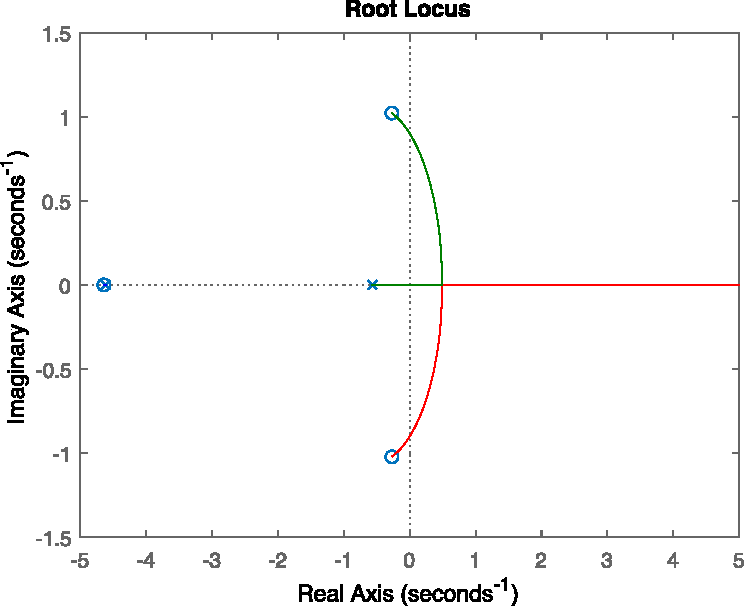
\includegraphics[scale=0.5]{figs/root_locus.pdf}
    \caption{Root locus for the linearized Rössler system.}
    \label{fig:root_locus}
\end{figure}


%%%%%%%%%%%%%%%%%%%%%%%%%%%%%%%%%%%%%%%%%%%%%%%%%%%

\subsection{Stability Analysis}

The following simulations were performed using the results from the Ruth-Hurwitz stability criterion. The first simulation, presented in Fig. \ref{fig:Ra_Dentro}, show the comparison between the original Rössler system and the linearization when changing the parameter $R_a$ inside the stability region, for three different values. Note that both systems show stable behavior but they do not present similar responses.

    \begin{figure}[ht]
        \centering
        \begin{subfigure}[b]{0.475\textwidth}
            \centering
            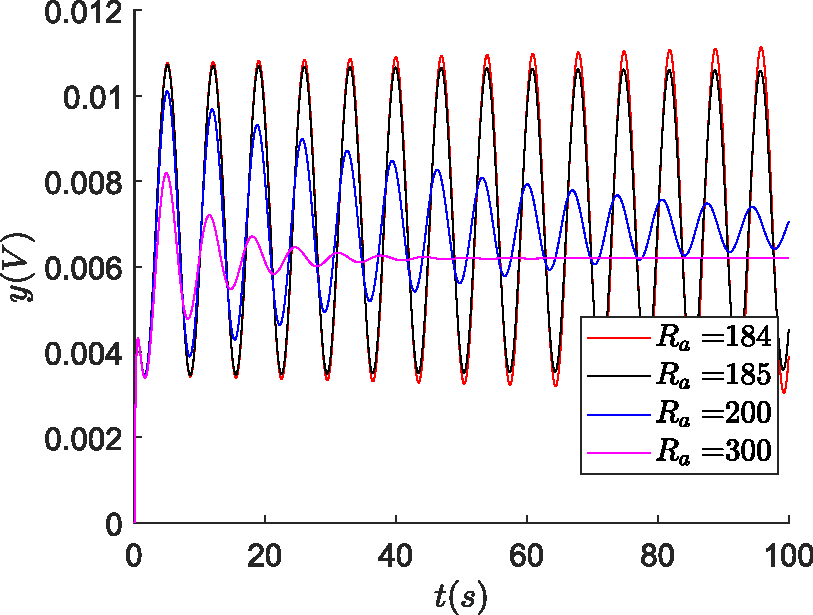
\includegraphics[scale=0.4]{figs/stab_Ra/Cambio_Ra_l_dentro.pdf}
            \caption{Linear.}
        \end{subfigure}
        \vskip0.1cm
        \begin{subfigure}[b]{0.475\textwidth}   
            \centering 
            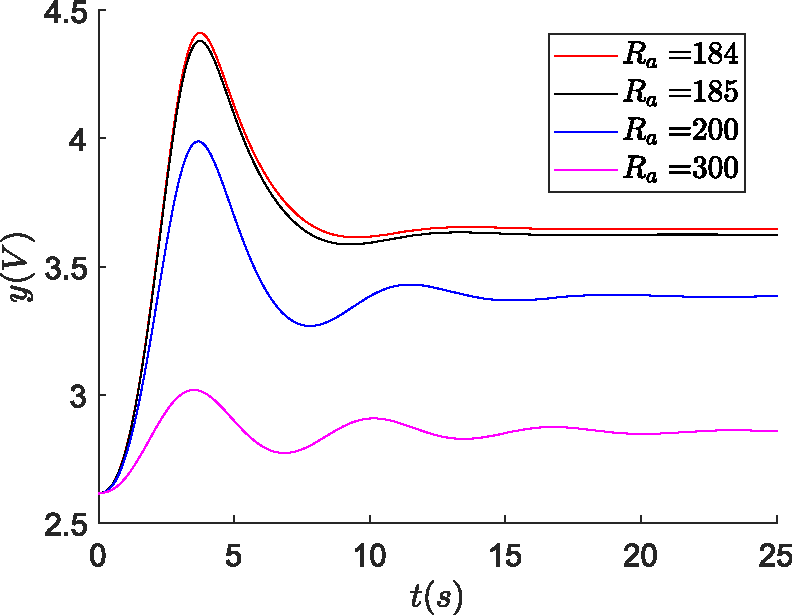
\includegraphics[scale=0.4]{figs/stab_Ra/Cambio_Ra_nl_dentro.pdf}
            \caption{Nonlinear.}
        \end{subfigure}
        \caption{Comparison for the linear and nonlinear systems for $R_a$ is the stability region.}
        \label{fig:Ra_Dentro}
	\end{figure}
	
	The second simulation was performed using three values for $R_a$ outside the stability region. The time responses for both the linear and nonlinear are shown in Fig. \ref{fig:Ra_Fuera}. 
	
	\begin{figure}[H]
        \centering
        \begin{subfigure}[b]{0.475\textwidth}
            \centering
            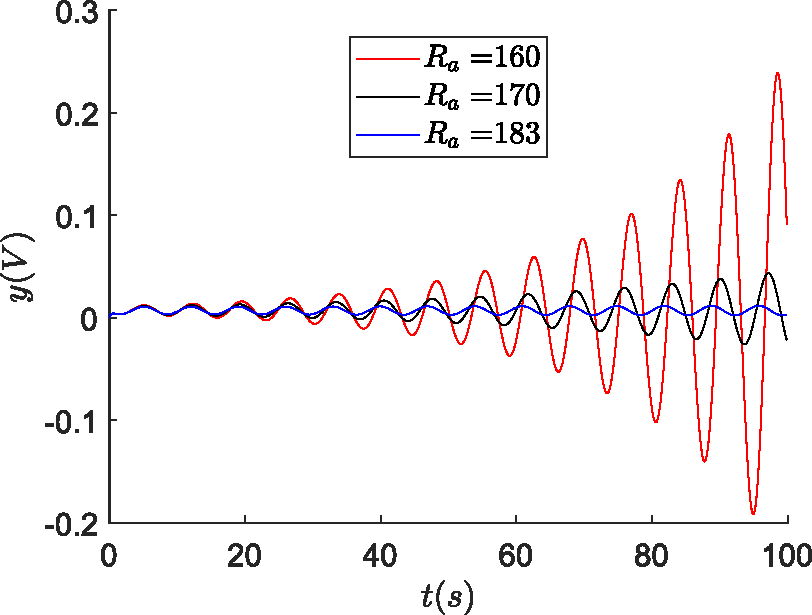
\includegraphics[scale=0.4]{figs/stab_Ra/Cambio_Ra_l_afuera.pdf}
            \caption{Linear.}
        \end{subfigure}
        \vskip0.1cm
        \begin{subfigure}[b]{0.475\textwidth}   
            \centering 
            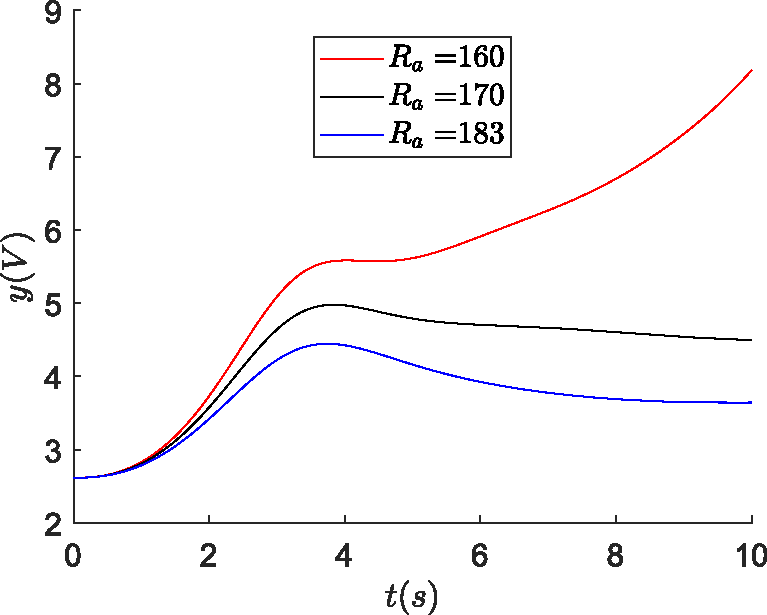
\includegraphics[scale=0.4]{figs/stab_Ra/Cambio_Ra_nl_afuera.pdf}
            \caption{Nonlinear.}
        \end{subfigure}
        \caption{Comparison for the linear and nonlinear systems for $R_a$ is the stability region.}
        \label{fig:Ra_Fuera}
	\end{figure}
	
	As it can be appreciated, the linear system shows a unstable behavior for all values, even though, for $R_a=183k\Omega$, it looks like it is critically stable. On the other hand, for the nonlinear system, the response is stable for values where the linear is unstable, and is unstable for $R_a=160k\Omega$.
	

%%%%%%%%%%%%%%%%%%%%%%%%%%%%%%%%%%%%%%%%%%%%%%%%%%%

\subsection{Bode Diagram}
The Bode diagram for the continuous system was obtained using \textit{Matlab} through the continuous transfer function (\ref{eq:tfNuestra}); in Fig. \ref{fig:contBode}.
\begin{figure}[ht]
    \centering
    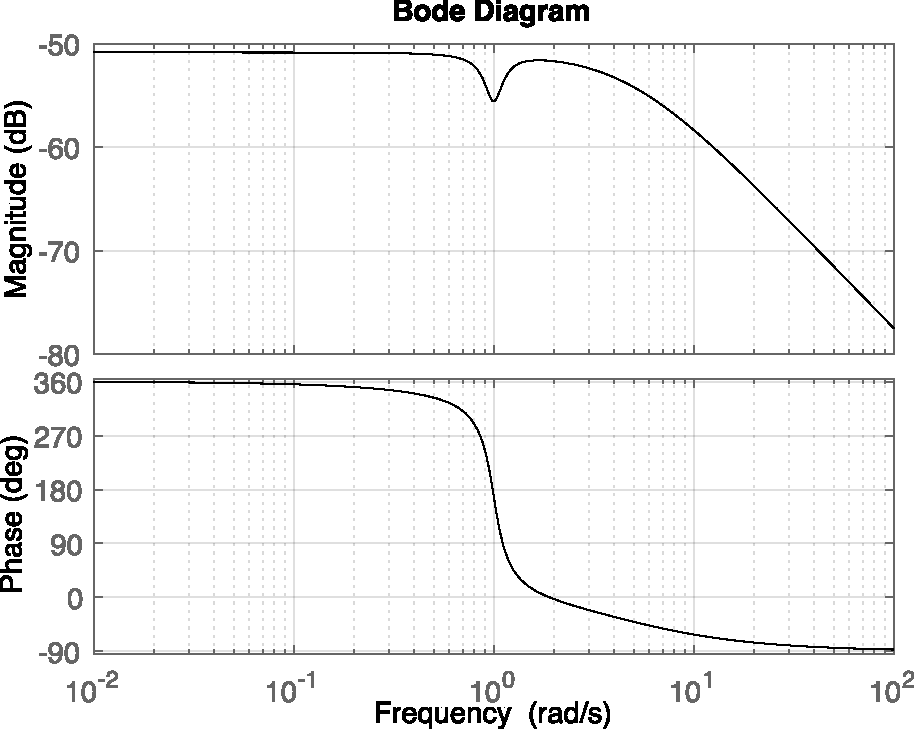
\includegraphics[scale=0.5]{figs/bodeDiagram.pdf}
    \caption{Bode diagram for the continuous linearized Rössler system.}
    \label{fig:contBode}
\end{figure}

The Bode diagram for the discrete system was calculated with \textit{Matlab} as well, using the discrete transfer function (\ref{eq:tfNuestraD}) and the obtained Bode diagram is shown in Fig. \ref{fig:discreteBode}.
\begin{figure}[ht]
    \centering
    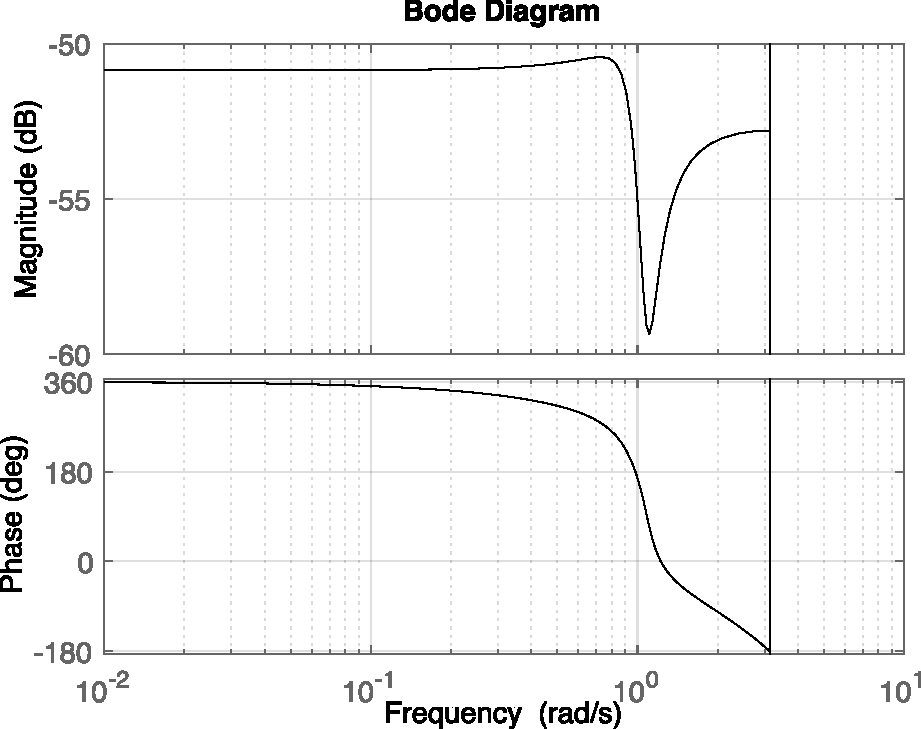
\includegraphics[scale=0.5]{figs/discreteBodeDiagram.pdf}
    \caption{Bode diagram for the discrete system.}
    \label{fig:discreteBode}
\end{figure}

As it was discussed in section \ref{sec:bode}, the Bode diagram can be used to determine the amplitude and phase for the output in stationary state, when the input is a sine wave. A simulation was conducted using a sine input with $A=1V$, $\omega=1rad/s$, hence
\begin{equation}\label{eq:inputFrequency}
    u(t)=(1V)\sin(t)
\end{equation}
From the Bode diagram, the respective amplitude relation and phase of the output in stationary state can be obtained. In Fig. \ref{fig:bodePoints} the respective phase and relative amplitude are shown. 
\begin{figure}[H]
    \centering
    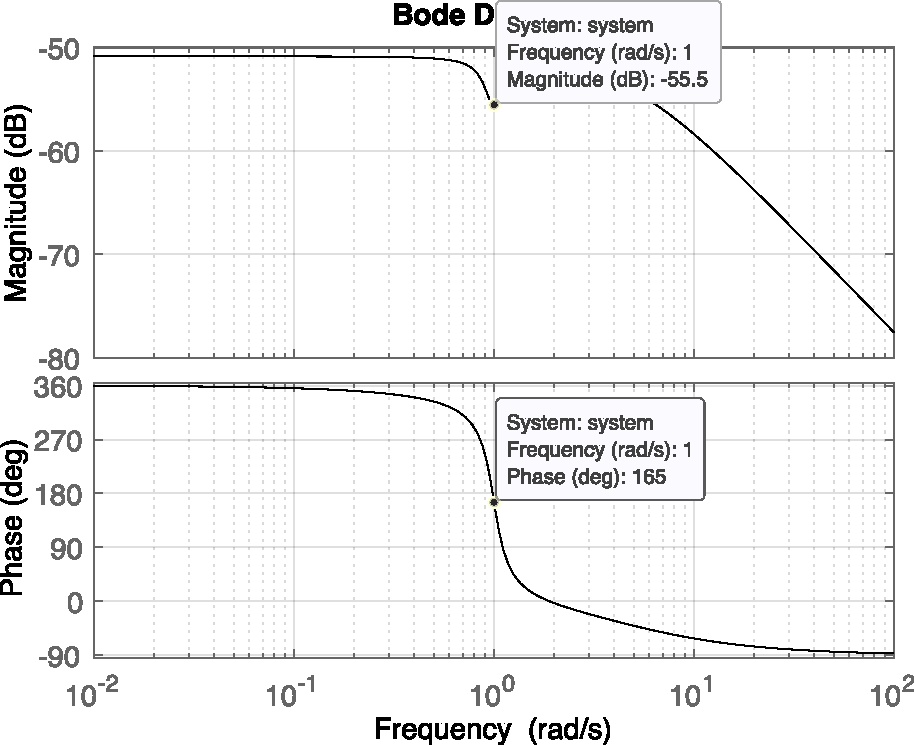
\includegraphics[scale=0.5]{figs/sineOutput/bodePointsW_1.pdf}
    \caption{Phase and relative amplitude for $\omega=1rad/s$.}
    \label{fig:bodePoints}
\end{figure}
Thus, the stationary state is given by
\begin{equation} \label{eq:sine_ss}
    y_{ss}(t)=0.0017\sin(t + 2.8798)
\end{equation}
In the following graph (Fig. \ref{fig:bode_sineOutput}), the system output to this input is shown, as well as the sine wave obtained for the stationary state. Note that the system, over time, adjusts to the expected sine wave.
\begin{figure}[H]
    \centering
    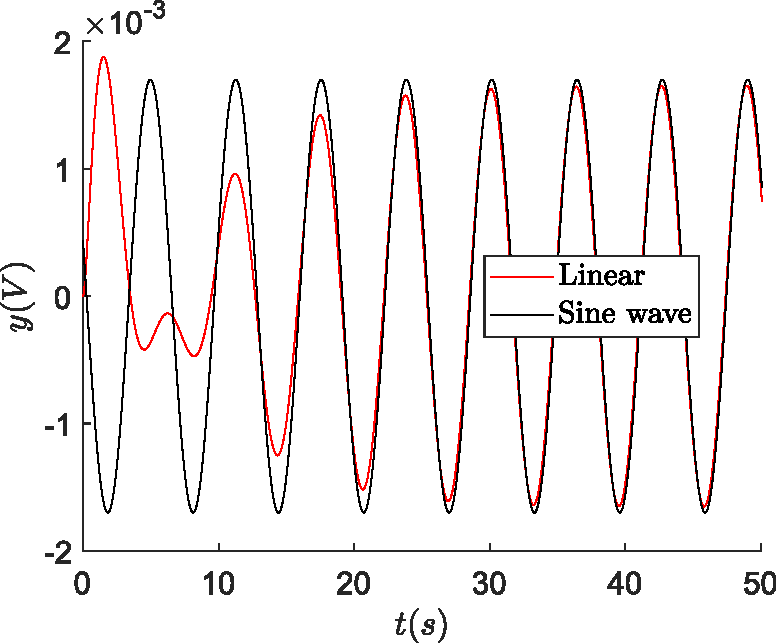
\includegraphics[scale=0.5]{figs/sineOutput/Entrada_seno_lineal_comparacion_bode.pdf}
    \caption{System output for sine input.}
    \label{fig:bode_sineOutput}
\end{figure}
%%%%%%%%%%%%%%%%%%%%%%%%%%%%%%%%%%%%%%%%%%%%%%%%%%%%%%

\subsection{Frequency Response Comparison with the Reduced Model}
The reduced model (\ref{eq:reduced_insignificant}) gave a good approximation to the original linear system, as it was proved through Fig. \ref{fig:reduced_insignificant}. In this section, this model is used to compare a frequency response in both systems; in order to achieve this, the Bode diagram for the reduced model was obtained, as shown in Fig. \ref{fig:bode_reducido}. 
\begin{figure}[H]
    \centering
    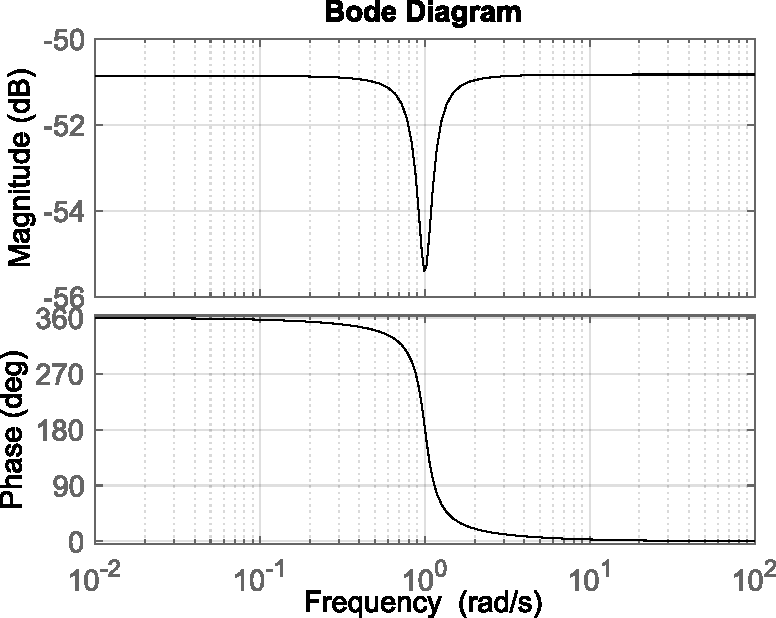
\includegraphics[scale=.5]{figs/sineOutput/Bode_reducido.pdf}
    \caption{Bode diagram for reduced order approximation.}
    \label{fig:bode_reducido}
\end{figure}


The selected input for the comparison was chosen as the same in equation (\ref{eq:inputFrequency}). Hence, a simulation was conducted an the results for the systems' responses are presented in Fig. \ref{fig:sinesOutput_Reduced}.

\begin{figure}[H]
    \centering
    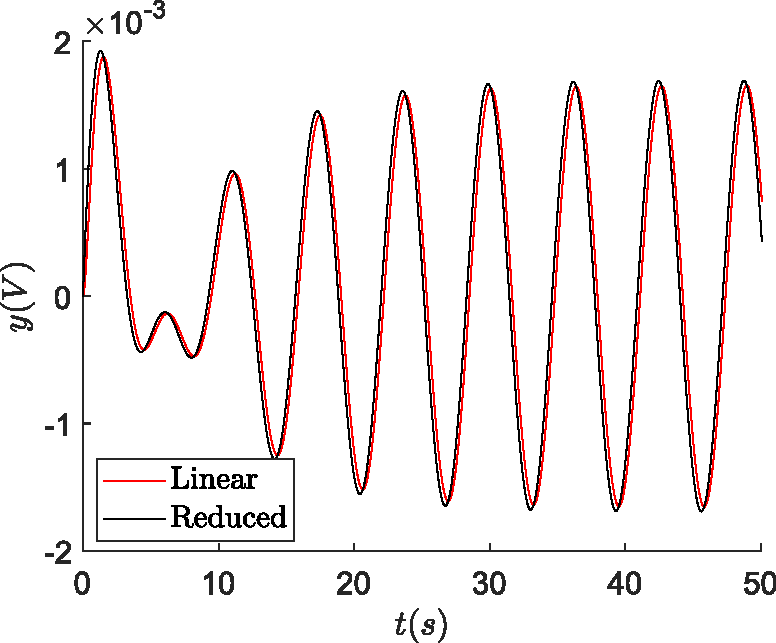
\includegraphics[scale=0.45]{figs/sineOutput/Comp_lin_red_seno.pdf}
    \caption{Comparison between outputs of the original model and the reduced for a sine wave input.}
    \label{fig:sinesOutput_Reduced}
\end{figure}
%%%%%%%%%%%%%%%%%%%%%%%%%%%%%%%%%%%%%%%%%%%%%%%%%%%%%%%%%%%%%
\subsection{Closed-Loop Stability}
The closed-loop stability analysis is based on the Bode diagram for the linearization of the Rössler system. The closed-loop diagram for this analysis is presented in Fig. \ref{fig:closedloop}. 
\begin{figure}[H]
    \centering
    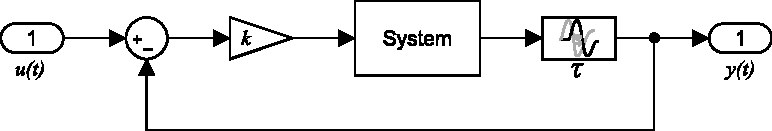
\includegraphics[scale=0.65]{figs/closedLoop.pdf}
    \caption{Closed-loop scheme.}
    \label{fig:closedloop}
\end{figure}

Using \textit{MATLAB}, as explained in \ref{sec:bode}, the gain margin and the phase margin were calculated obtaining a maximum value for the gain of the closed-loop system of $k_{max} = 601.2835$ to preserve a stable system. On the other hand, it was found that a delay can not unstabilize the linear Rössler system. This first simulation, in Fig. \ref{fig:response_gains_k}, the $k$ was selected for three different values inside the stability region.

\begin{figure}[ht]
    \centering
    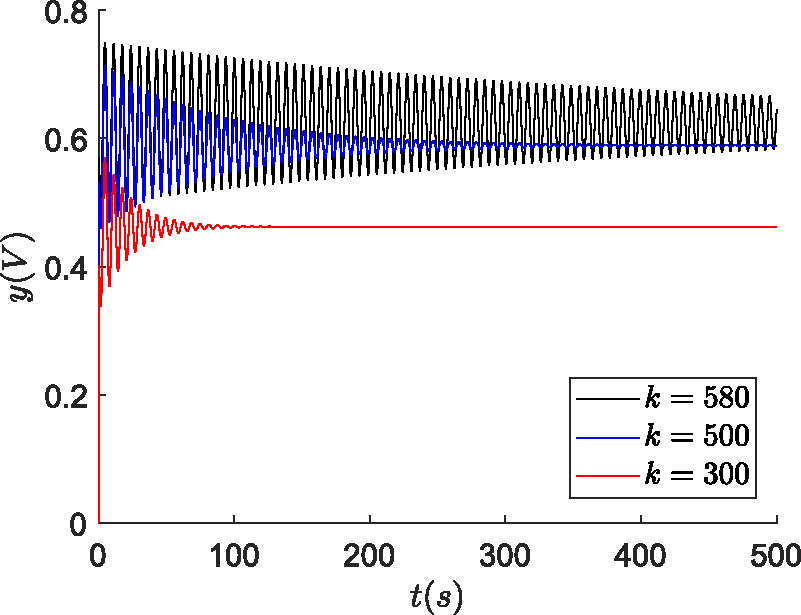
\includegraphics[scale=0.5]{figs/sineOutput/Lazo_cerrado_estable.pdf}
    \caption{Stable system's response to some gains.}
    \label{fig:response_gains_k}
\end{figure}

The following simulation, in Fig. \ref{fig:response_gains_unstable}, it was selected three different values for $k$ outside the stability region. It is important to notice that for $k=620$ it does not seem as it had any unstable behaviour as for the other values chosen; this will be explained in \ref{sec:resultAn}.

\begin{figure}[H]
    \centering
    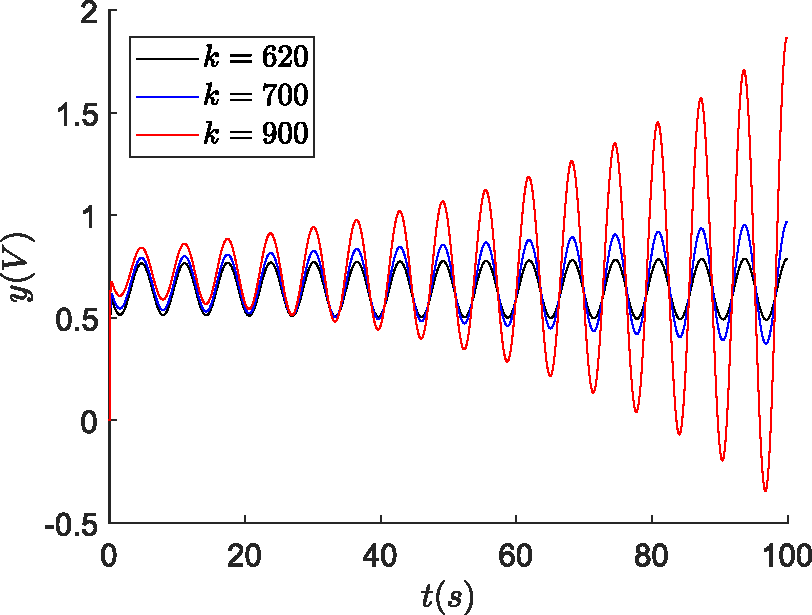
\includegraphics[scale=0.5]{figs/sineOutput/Lazo_cerrado_inestable.pdf}
    \caption{Unstable system's response to some gains.}
    \label{fig:response_gains_unstable}
\end{figure}

Lastly, in Fig. \ref{fig:response_delays}, the closed-loop system was simulated with three different delays. As predicted by the margins calculated, the delay does not unstabilize the system.

\begin{figure}[H]
    \centering
    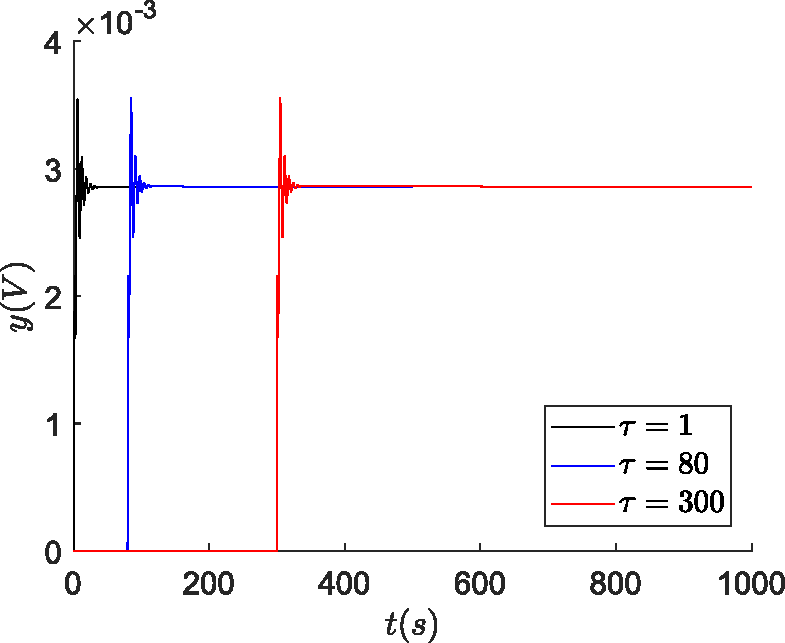
\includegraphics[scale=0.5]{figs/sineOutput/Lazo_cerrado_retardo.pdf}
    \caption{System's response to some delays.}
    \label{fig:response_delays}
\end{figure}
